\section{Data processing}\label{sec:processing}

The PD signal is amplified by a computer-controlled variable pre-amplifier to use the full
range of the AD converter. The absolute gain and the offset have no influence on the
measurement accuracy, it is only necessary to provide a linear response. Since the reflectivity
R is encoded in only one optical/electrical signal the constraints on the amplifier have become
negligible. This is in contrast to the method of Haiml et al., in which the same gain and no
offset has to be achieved by both amplifiers [16].
The computer algorithm first detects the rising edges (red dots in Fig. 4(c)) and then takes
the mean value of the data points on the flat levels (red lines in Fig. 4(b)). As both beams are
blocked in phase 4, we can precisely measure the offset of the photodiode. Level A and B
(Fig. 4(b)) are obtained by subtracting the signal level in state 1, and the nonlinear reflectivity
is obtained as R = B / A. This is done for 500 periods in succession (takes approximately 5
seconds per fluence) and averaged to minimize detector noise and laser noise. This averaged
reflectivity has a standard deviation of 0.01\%. The incident fluence can be computed from the
level A and the pre-amplifier gain setting. An accuracy of 5\% for the fluence measurement is
typically good enough, as this will afterwards result in an inaccuracy of 5\% for the fitted
saturation fluence Fsat.

\begin{figure}[ht]
    \centering
    \sidesubfloat[]{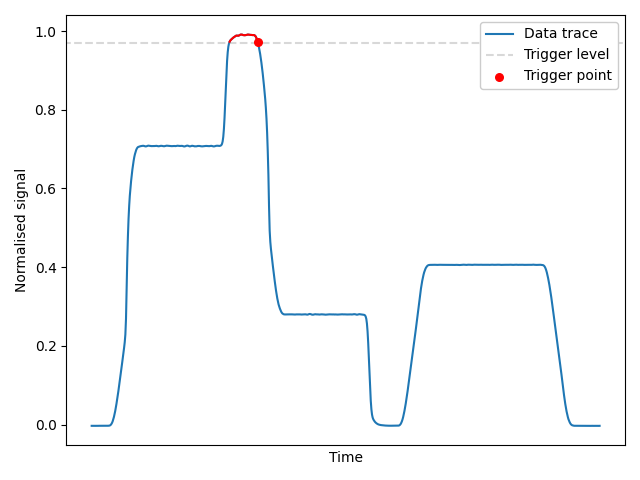
\includegraphics[width=0.29\linewidth]{images/old_trace.png}\label{fig:a}}
    \sidesubfloat[]{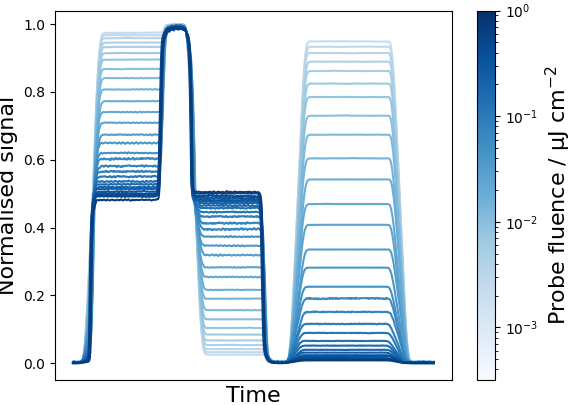
\includegraphics[width=0.29\linewidth]{images/trace_complete.png}\label{fig:b}}
    \sidesubfloat[]{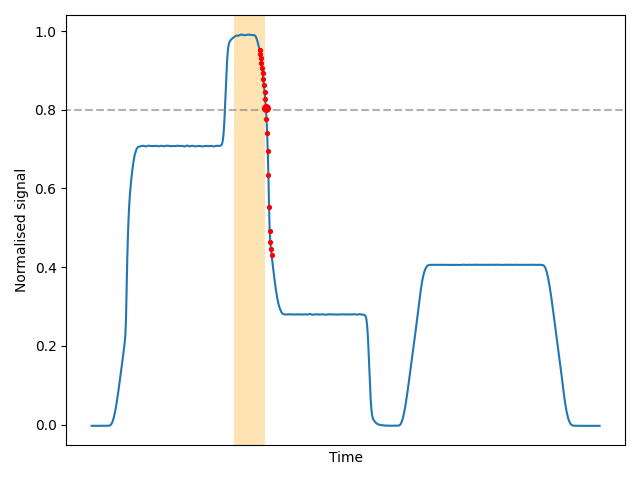
\includegraphics[width=0.29\linewidth]{images/corrected_signal.png}\label{fig:c}}
    \caption{Main caption}
\end{figure}